\chapter{پیاده‌سازی}
در بخش قبلی معماری کلی سیستم و ماژول‌های موردنیاز برای پیاده‌سازی سیستم ردیابی را بیان و به صورت اجمالی معرفی کردیم. در این فصل به چگونگی قرار گرفتن و ارتباط بخش‌های مختلف می‌پردازیم و پیاده‌سازی سیستم را توضیح خواهیم داد.


سیستم ردیابی طراحی شده در این پروژه از ماژول آردوینو و سیم ۸۰۸ که شامل آنتن جی‌اس‌ام و جی‌پی‌اس می‌باشد، برای ردیابی استفاده می‌کند. هسته اصلی این پروژه میکروکنترلر آردوینو می‌باشد. موقعیت جغرافیایی شی تویط آنتن جی‌پی‌اس دریافت شده و سپس این اطلاعات با استفاده از تکنولوژی جی‌اس‌ام به وب سرور فرستاده می‌شود. برای مشاهده کردن و ردیابی شی بر روی نقشه، یک برنامه کاربردی تحت وب توسعه داده شده است. این برنامه کاربردی به زبان \lr{PHP}، \lr{HTML} نوشته شده و از نرم‌افزار \lr{WampServer} برای اجرای آن استفاده می‌شود.
 
 
در ابتدا ماژول سیم ۸۰۸ برای گرفتن موقعیت مکانی از ماهواره مقداردهی اولیه می‌شود. تنظیمات اولیه این دستگاه با استفاده از دستورات \lr{AT} انجام می‌شود. با متصل کردن آنتن چی‌پی‌اس این ماژول قادر خواهد بود مختصات مکانی را از ماهواره دریافت کند. سپس تنظیمات مربوط به شبکه جی‌پی‌آر‌اس انجام می‌شود.


آنتن‌های جی‌اس‌ام و جی‌پی‌اس به ماژول سیم ۸۰۸ متصل می‌شوند. برد آردوینو و ماژول سیم ۸۰۸ دارای پین اتصال به زمین مشترک هستند. برنامه نوشته شده به زبان سی بر با استفاده از نرم‌افزار \lr{Arduino IDE} روی برد آردوینو آپلود می‌شود.
\\
در شکل ۴-۱ نحوه اتصال ماژول‌های مختلف در سیستم ردیابی نشان داده شده است:
\begin{figure}[!h]
	\centerline{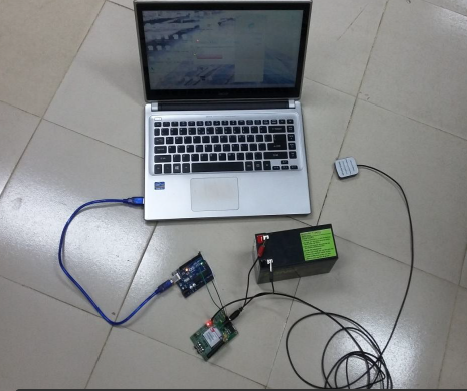
\includegraphics[width=.6\textwidth]{design-system}}
	\caption{سیستم ردیابی طراحی شده}
\end{figure}
\section{بررسی عملکرد سیستم ردیابی}
همانطور كه گفته شد، قسمت سخت‌ افزاری سیستم ما از چهار ماژول سیم ۸۰۸، گیرنده جی‌اس‌ام، گیرنده جی‌پی‌اس و میکروکنترلر آردوینو تشکیل شده است. در اين قسمت، پياده‌سازي سيستم طراحی شده، شيوه ارتباط اجزای مختلف و كد پياده‌سازي شده را توضيح خواهیم داد.
\subsection{بررسی عملکرد مدار}
پيش از پرداختن به ماژول‌ها و شيوه اتصال آن‌ها، لازم است شيوه عملكرد ميكروكنترلر سيستم و نحوه پردازش اطلاعات را در فلوچارتي مشاهده كنيم. عملكرد كلي سيستم در بخش قبل توضيح داده شد. اكنون با ارئه فلوچارتي درباره الگوريتم پياده‌سازي شده می‌توانیم درك بهتري نسبت به روند كار در مدار سخت‌افزاری طراحی شده و كد نوشته شده براي آن داشته باشيم.

\newpage
فلوچارت شكل ۴-۲ روند كلي كد پياده‌سازي شده بر روي آردوینو را نمايش می‌دهد.
\begin{figure}[h!]
	\centering
	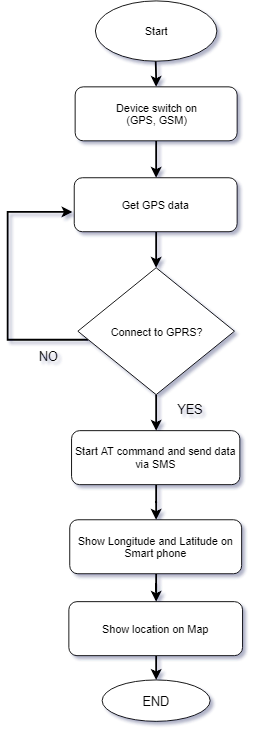
\includegraphics[width=.4\textwidth]{tracking-flowchart}
	\caption{عملکرد کد پیاده‌سازی شده بر روی آردوینو \cite{Rahman2016,Alshamsi,Hazza}}
\end{figure}
\\


در ابتدای کار برای تست سیستم طراحی شده، آنتن جی‌پی‌اس به ماژول سیم ۸۰۸ متصل می‌شود تا موقعیت مکانی (طول و عرض جغرافیایی) شی را از ماهواره دریافت کند. برای انجام این کار از نرم‌افزار \lr{Arduino IDE} برای پروگرم کردن کد نوشته شده بر روی برد آردوینو استفاده می‌شود.\\
\\
در فلوچارت شکل ۴-۳ نحوه کار جی‌پی‌اس نشان داده شده است.
\begin{figure}[!h]
	\centerline{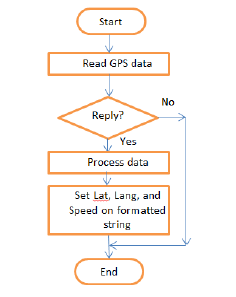
\includegraphics[width=.3\textwidth]{gps-flowchart}}
	\caption{فلوچارت خواندن اطلاعات \lr{GPS} \cite{ElShafee2013}}
\end{figure}


برای ارسال موقعیت مکانی شی به کاربر از طریق شبکه جی‌اس‌ام از ماژول سیم ۸۰۸ و میکروکنترلر آردوینو متصل به آن استفاده می‌شود. برای ارتباط ماژول سیم ۸۰۸ با شبکه جی‌اس‌ام از دستورات \lr{AT} برای برنامه‌نویسی و کنترل آن استفاده می‌کنیم.
\\
در فلوچارت شکل ۴-۴ نحوه کار \lr{GSM} نشان داده شده است.
\begin{figure}[!h]
	\centerline{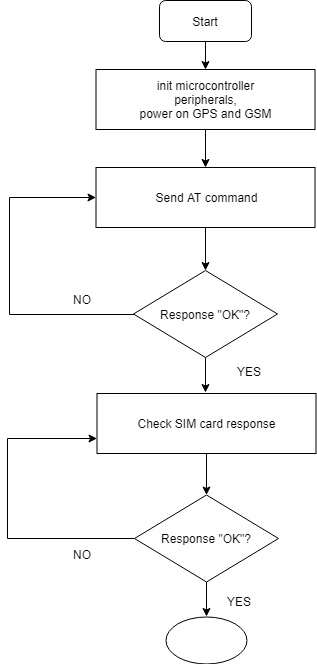
\includegraphics[width=.3\textwidth]{gsm-flowchart}}
	\caption{فلوچارت نحوه کار \lr{GSM} \cite{ElShafee2013}}
\end{figure}
\begin{figure}[!h]
	\centerline{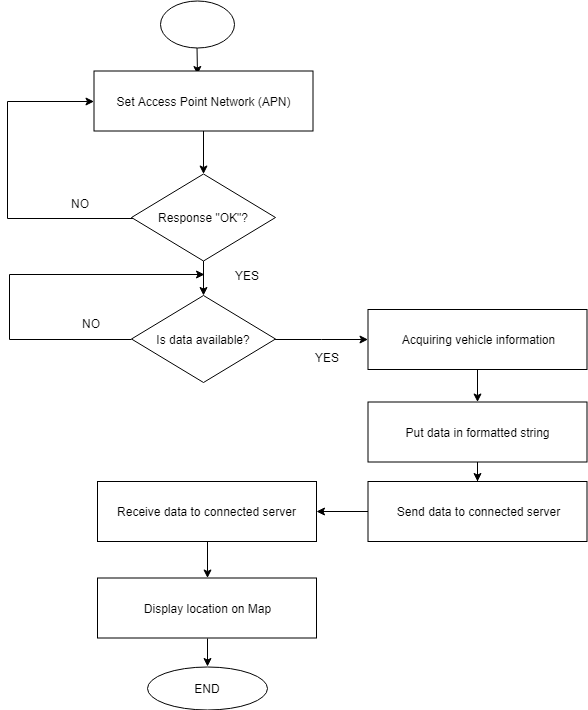
\includegraphics[width=.4\textwidth]{continue-gsm}}
	\caption{ادامه فلوچارت نحوه کار \lr{GSM} \cite{ElShafee2013}}
\end{figure}


سیستم ردیابی طراحی شده متشکل از ماژول سیم ۸۰۸ متصل به برد آردوینو می‌باشد. این ماژول دستور \lr{AT} را می‌فرستد، اگر جواب این دستور \lr{OK} باشد وضعیت شبکه چک می‌شود. بعد از چک شدن وضعیت شبکه و وصل شدن به آن، وضعیت جی‌پی‌اس چک شده و موقعیت مکانی شی از آن دریافت می‌شود. پس از دریافت اطلاعات جغرافیایی، درخواست ارسال اطلاعات به سرور ارسال می‌شود. در انتها داده ارسال شده در سمت سرور به وسیله اسکریپت نوشته پردازش شده و موقعیت شی بر روی نقشه نشان داده خواهد شد.
\\
در فلوچارت شکل ۴-۶ فلوچارت اسکریپت \lr{PHP} نشان داده شده است.

\begin{figure}[h!]
	\centering{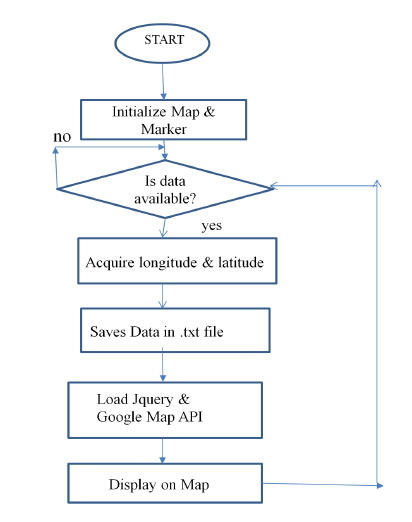
\includegraphics[width=.3\textwidth]{php-flowchart}}
	\caption{فلوچارت فایل  \lr{PHP} \cite{ElShafee2013}}
\end{figure}
\section{بررسی معماری مدار}
در این قسمت بخش سخت‌ افزاری سیستم پیشنهادی را توضیح می‌دهیم. همانطور که در قسمت‌های قبل مشخص شد، با استفاده از آنتن جی‌ پی اس متصل به ماژول سیم ۸۰۸ اطلاعات مربوط به موقعیت مکانی شی از ماهواره دریافت شده و سپس از طریق شبکه جی اس ام به سرور فرستاده می‌شود. در شکل ۴-۷ شیوه اتصال ماژول سیم ۸۰۸ به آردوینو را مشاهده می‌کنید.
\\
\begin{figure}[!h]
	\centerline{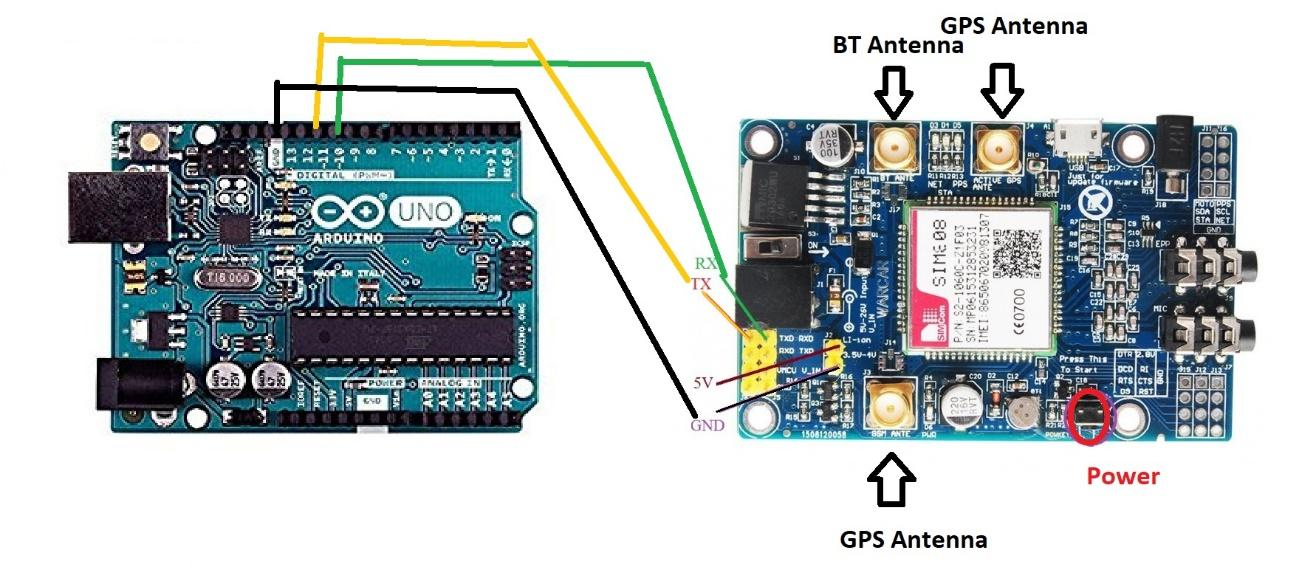
\includegraphics[width=.6\textwidth]{sim808-arduino}}
	\caption{شیوه اتصال آردوینو به ماژول سیم ۸۰۸\cite{interface}}
\end{figure}


ماژول سیم ۸۰۸ با استفاده از رابط سریال به آردوینو متصل شده است، دارای دو پایه \lr{TX} و \lr{RX} است که به ترتیب به پایه دیجیتال ۱۰ و ۱۱ آردوینو متصل شده‌اند. پایه اتصال به زمین این ماژول هم به پایه اتصال به زمین برد آردوینو متصل شده است. ولتاژ موردنیاز ماژول سیم ۸۰۸ را از طریق آداپتور ۹ ولت خروجی تامین می‌کنیم. 
\section{برنامه کاربردی}